%!TEX root = ../../dissertation.tex


\section{VR Azuchi Castle} % (fold)
\label{sec:vr_azuchi_castle}


In \cite{fukuda2015}, Tomohiro Fukuda et al, presented a \gls{HD} \gls{VR} system for Historical Architectural and Urban Digital Reconstruction. They used the Azuchi Castle and the surrounding town as case study. 

They have the goal of having a real time rendering system with high accuracy and realism. With that, they face the same problems as we did. In \cite{fukuda2015}, is consider the problem of rendering large sets of objects of different scales in real time. It is also presented the various techniques they used to face this problem.

\begin{figure}[htbp]
	\centering
	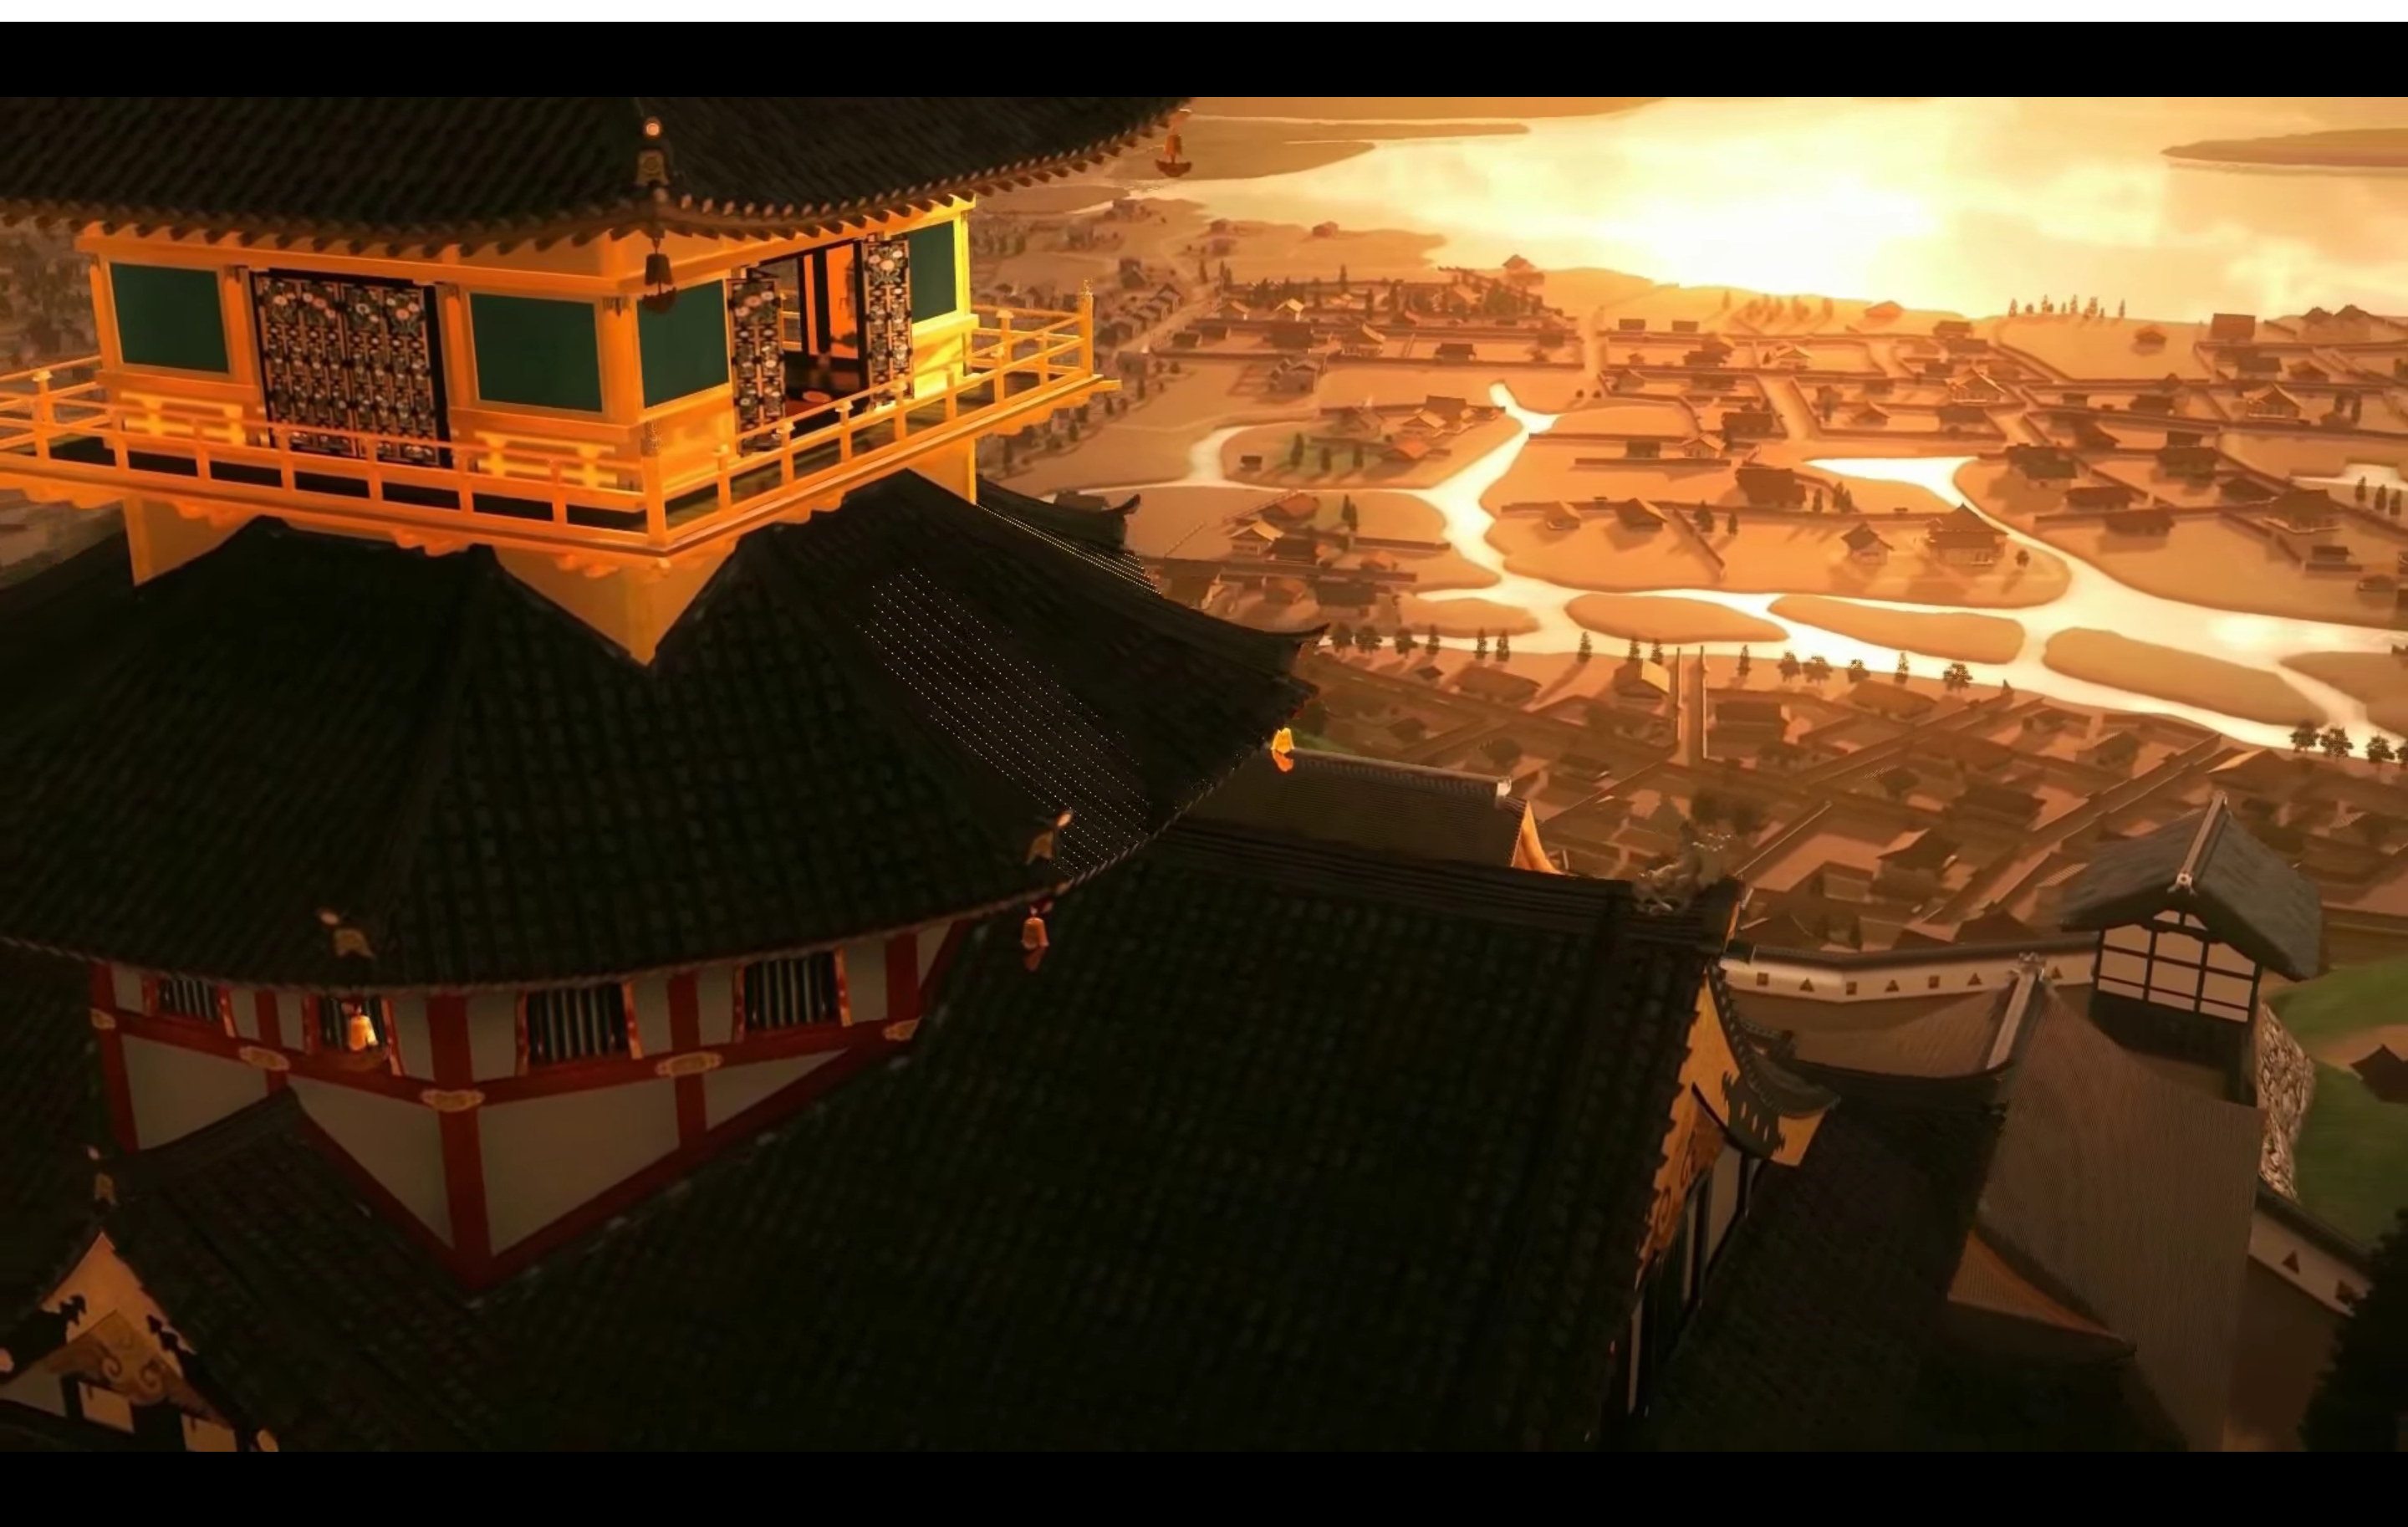
\includegraphics[width=0.95\textwidth]{images/azuchi/view.png}
	\caption{Azuchi castle view}
	\label{fig:azichiview}
\end{figure}

(...)

% section vr_azuchi_castle (end)
		